\section{eo\-Fl\-Or1pt\-Quad\-Op$<$ EOT $>$ Class Template Reference}
\label{classeo_fl_or1pt_quad_op}\index{eoFlOr1ptQuadOp@{eoFlOr1ptQuadOp}}
The 1pt crossover (just in case someone wants it some day!).  


{\tt \#include $<$eo\-Fl\-Or\-Quad\-Op.h$>$}

Inheritance diagram for eo\-Fl\-Or1pt\-Quad\-Op$<$ EOT $>$::\begin{figure}[H]
\begin{center}
\leavevmode
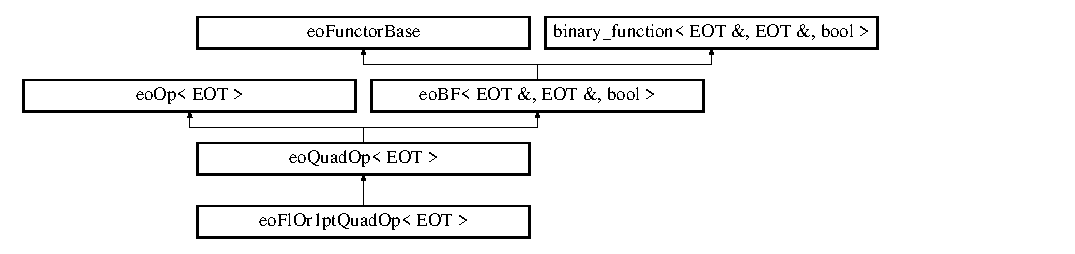
\includegraphics[height=2.96296cm]{classeo_fl_or1pt_quad_op}
\end{center}
\end{figure}
\subsection*{Public Types}
\begin{CompactItemize}
\item 
typedef EOT::Atom\-Type {\bf Atom\-Type}\label{classeo_fl_or1pt_quad_op_w0}

\end{CompactItemize}
\subsection*{Public Member Functions}
\begin{CompactItemize}
\item 
{\bf eo\-Vl\-Uniform\-Quad\-Op} ()\label{classeo_fl_or1pt_quad_op_a0}

\begin{CompactList}\small\item\em default ctor: no argument \item\end{CompactList}\item 
bool {\bf operator()} ({\bf EOT} \&\_\-eo1, {\bf EOT} \&\_\-eo2)\label{classeo_fl_or1pt_quad_op_a1}

\begin{CompactList}\small\item\em exchanges first and second parts of the vectors of Atoms \item\end{CompactList}\item 
virtual string {\bf class\-Name} () const \label{classeo_fl_or1pt_quad_op_a2}

\begin{CompactList}\small\item\em inherited {\bf class\-Name()}{\rm (p.\,\pageref{classeo_fl_or1pt_quad_op_a2})} \item\end{CompactList}\end{CompactItemize}


\subsection{Detailed Description}
\subsubsection*{template$<$class EOT$>$ class eo\-Fl\-Or1pt\-Quad\-Op$<$ EOT $>$}

The 1pt crossover (just in case someone wants it some day!). 



Definition at line 173 of file eo\-Fl\-Or\-Quad\-Op.h.

The documentation for this class was generated from the following file:\begin{CompactItemize}
\item 
eo\-Fl\-Or\-Quad\-Op.h\end{CompactItemize}
